\section{Introduction}
\label{sec:introduction}
\begin{itemize}
    \item Mechanical computing uses deformation and mechanical motion for data storage and computation.
    \item Applicable in intelligent mechanical systems like soft devices, MEMS, and robotic materials.
    \item Limitation: Inefficient data exchange between memory and computing modules hampers performance.
    \item Logic gates realized through origami, buckled beams, and mechanical linkages.
    \item Signal propagation via mechanical, mechano-electronic, and mechanical-fluidic interfaces.
    \item Non-volatile mechanical memory exists but requires complex peripherals or intricate energy landscapes.
    \item Consideration: Cellular automata as a potential architecture to address data exchange bottleneck.
\end{itemize}
\section{Results}

\subsection*{Elementary Cellular Automata Formalism}
Cellular automata (CA) are grid-based computational models where each cell evolves over time according to a rule set \( R \). In Elementary Cellular Automata (ECA), the domain is one-dimensional and the state space is binary, \( S = \{0, 1\} \). Each cell's future state is determined by its current state and those of its immediate neighbours.

Mathematically, for cell \( i \) at time \( t \), the next state \( u_i^{t+1} \) is governed by a rule function \( f: S^3 \to S \):

\[
u_i^{t+1} = f(u_{i-1}^t, u_i^t, u_{i+1}^t)
\]

With a binary state and 3-cell neighbourhood, there are \( 2^8 = 256 \) unique ECA rules. These are indexed from 0 to 255, following Wolfram's convention, detailed in \autoref*{sec:Wolfram Numbering Scheme for ECA}.

For example, Rule 110 is defined explicitly as:
\[
\begin{array}{ll}
f_{\text{110}}: & (0,0,0) \to 0, \; (0,0,1) \to 1, \; (0,1,0) \to 1, \; (0,1,1) \to 1, \\
& (1,0,0) \to 0, \; (1,0,1) \to 1, \; (1,1,0) \to 1, \; (1,1,1) \to 0
\end{array}
\]

Consult \autoref{fig:cube}A for a graphical depiction of Rule 110's eight possible neighbourhoods and their respective output states. Also shown is the time evolution of the rule, starting from a single 'on' cell at the left edge of the domain.

\subsection*{Hypercube Representation of Cellular Automata Rules}
Consider a cube in \( \mathbb{R}^3 \) as the domain \( D \), with each vertex representing a unique neighbourhood configuration \( N = (N_{-1}, N_0, N_1) \), where \( N_{-1}, N_0, N_1 \in \{0, 1\} \). The cube's vertices are colored based on a rule function \( f: \{0, 1\}^3 \to \{0, 1\} \), thereby geometrically realizing the Boolean truth table of an Elementary Cellular Automaton (ECA).

To introduce the concept of linear separability, consider separating parallel hyperplanes \( P \) defined by a normal vector \( \mathbf{n} \) and offsets \( \{d_1, d_2, \ldots, d_n\} \). These hyperplanes partition \( D \) into regions where the vertices share the same output state as determined by \( f \).

We define a domain classification function \( \Delta: D \to \{0, 1, \ldots, n\} \) as \( \Delta(x) = \sum_{i=1}^{n} H(\mathbf{n} \cdot \mathbf{x} - d_i) \), where \( H(z) \) is the Heaviside step function. Each value of \( \Delta(x) \) corresponds to one of the \( n+1 \) regions formed by \( P \).

Finally, a mapping function \( M: \{0, 1, \ldots, n\} \to \{0, 1\} \) translates the region identifier \( \Delta(x) \) into the 'on' or 'off' state for each neighbourhood configuration.
Refer to \autoref*{fig:cube}B for a graphical representation of the cube and separating planes for Rule 110.

As shown in Appendix \ref*{sec:Bi-planar separability of ECA rules}, most ECA rules are bi-planarly separable, i.e. they can be represented by two parallel planes. 


\begin{figure}[ht]
    
    \centering
    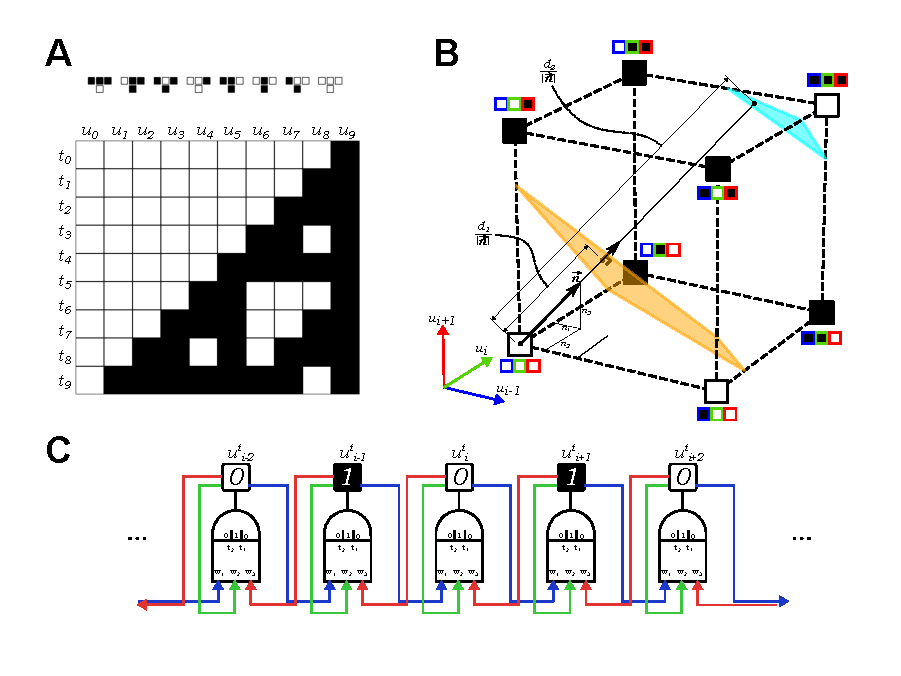
\includegraphics[width=\textwidth]{images/SVGs/Cube.pdf}
    \caption{A. The transition rule and time evolution of the Rule 110 cellular automata. B. Cube representation Rule 110 with separating planes defined by normal vector $\overrightarrow{n}$ and offset constants $d_1$ and $d_2$. The red, green and blue colouring corresponds to left neighbour, middle, and right neighbour cells of the neighbourhood respectively. C. Bi-threshold gate representation of an ECA architechture.}
    \label{fig:cube}
\end{figure}

% \subsection*{Bi-threshold Gates}

The result of this formulation of 3-input Boolean functions as linearly separable regions in a cube is the observation that most 3-input Boolean functions can be represented by a pair of parallel planes. This means we can translate a complicated Boolean algebraic expression composed of several AND, OR, XNOR, etc., gates into a single bi-threshold perceptron gate.

The bi-threshold perceptron for this ECA context can be formally represented as:

\[
f(N) = \begin{cases} 
0 & \text{if } \sum_{i=-1}^{1} w_i \cdot N_i > T_1 \\
1 & \text{if } T_2 \leq \sum_{i=-1}^{1} w_i \cdot N_i \leq T_1 \\
0 & \text{if } \sum_{i=-1}^{1} w_i \cdot N_i < T_2
\end{cases}
\]


\subsection*{Concept Mechanism}

In light of the mathematical formalism presented, we introduce a conceptual mechanical metamaterial designed to embody the logic and behavior of Elementary Cellular Automata (ECAs). This metamaterial is constructed from an array of interconnected unit cells, each serving as a mechanical analog to the bi-threshold pergeptron gate.

The core of each unit cell is a tristable element, functioning as the decision-making component. The tristable element has three stable states, akin to the three regions separated by the two parallel planes in the cube of our geometric representation. This element is responsible for holding the output state of the cell, dictated by the weighted sum of its inputs. 

Each unit cell is interconnected via coupling springs, which transmit mechanical signals between adjacent cells. The stiffness values of the coupling springs \(k_i\) act as the weights \( w_i \) in the bi-threshold perceptron equation. These values determine the force interactions and state transitions between adjacent unit cells. The tristable elements have multiple stable states, analogous to the regions separated by planes in the cube of our geometric ECA representation.

An input clock signal introduces a temporal dimension to the mechanical system, enabling dynamic state evolution similar to time-stepping in ECAs. This clock signal sets the computational cycle and synchronizes the unit cells.

Thus, the mechanical properties of the springs and tristable elements correspond directly to the mathematical constructs of the bi-threshold perceptron, providing a means to implement ECA rules in a mechanical system. The specific embodiment of this concept is detailed in the following section.

\subsection*{Unit cell design}
The unit cell is designed to be planar and monolithic for scalability, operate under a single shared clock signal for synchronization, transmit forces between adjacent cells, hold state in the absence of input, and transition states according to neighboring conditions. \autoref*{fig:Mechanism}A depicts the unit cell and its key components: the tristable element in teal, the bistable element in purple, the signal transmission element in orange, and the input bifurcation element in dark blue. Coupling springs, coloured in red, green, and blue, link the tristable element out-of-plane to the bifurcation elements of adjacent unit cells. The configuration of each unit cell is fully defined by two displacements: \(d^t\) in the \(\hat{e}_1\) direction for the tristable element and \(d^b\) in the \(\hat{e}_1\) direction for the bifurcation element ldue to the parallel links constraining rotational degrees of freedom. The input bifurcation element is so named because under actuation by an input clock signal \(\epsilon\), its shuttle block will displace a distance \(\delta\) in one of two directions, pushing or pulling on the coupling springs according to the state of the unit cell, "on" or "off" respectively. In order for the the bifurcation element to bifurcate only due to the configuration of the bistable element and not the tristable element, the operation of the unit cell requires the coupling springs to be \emph{tension-only} (\autoref*{fig:Mechanism}B). The details of this feature is elaborated in the next section. 

The bistable element acts as a mechanical binary memory element for the unit cell, while the tristable element's two snapthrough force thresholds act as decision boundaries corresponding to the thresholds of the threshold gate, or the separating planes of the boolean function. The signal transmission and bifurcation elements facilitate the temporal clocking and informational interconnection of the unit cells. 

A simplified pseudo-rigid body model of the unit cell is depicted in Figure \autoref*{fig:Mechanism}B. In this model, the contributions of numerous short-length flexure joints are aggregated into four torsional springs with angular stiffnesses \((k_\alpha, k_\beta, k_\gamma, k_\theta)\). These springs are subject to characteristic angular displacements \((\alpha, \beta, \gamma, \theta)\), which represent the angles of the tristable, bistable, signal transmission, and bifurcation links, respectively. The angles \(\alpha\), \(\beta\), and \(\gamma\) are part of a single-degree-of-freedom kinematic chain, while \(\theta\) and the input displacement \(\epsilon\) form another single-degree-of-freedom kinematic chain.
The bistable element is simplified using symmetry and modeled as a single-link slider with torsional stiffness \( k_\beta \) and a reaction/support stiffness \( k_r \). The transmission element is represented as a single link connecting the bistable element's shuttle block to a horizontal slider block. This link has a torsional stiffness \( k_\gamma \) and is guided by flexures with a support stiffness \( k_g \).
The signal transmission block is connected to the bifurcation element via a spring with stiffness \( k_s \). This spring is attached at a point located a distance \( h \) from the anchor pivot of the bifurcation element.
\todo{add h to figure}

\autoref*{fig:Mechanism}C shows the effect of the position of the tristable element on the behaviour of the bifurcation element under actuation. 


\begin{figure}[h]
    \centering
    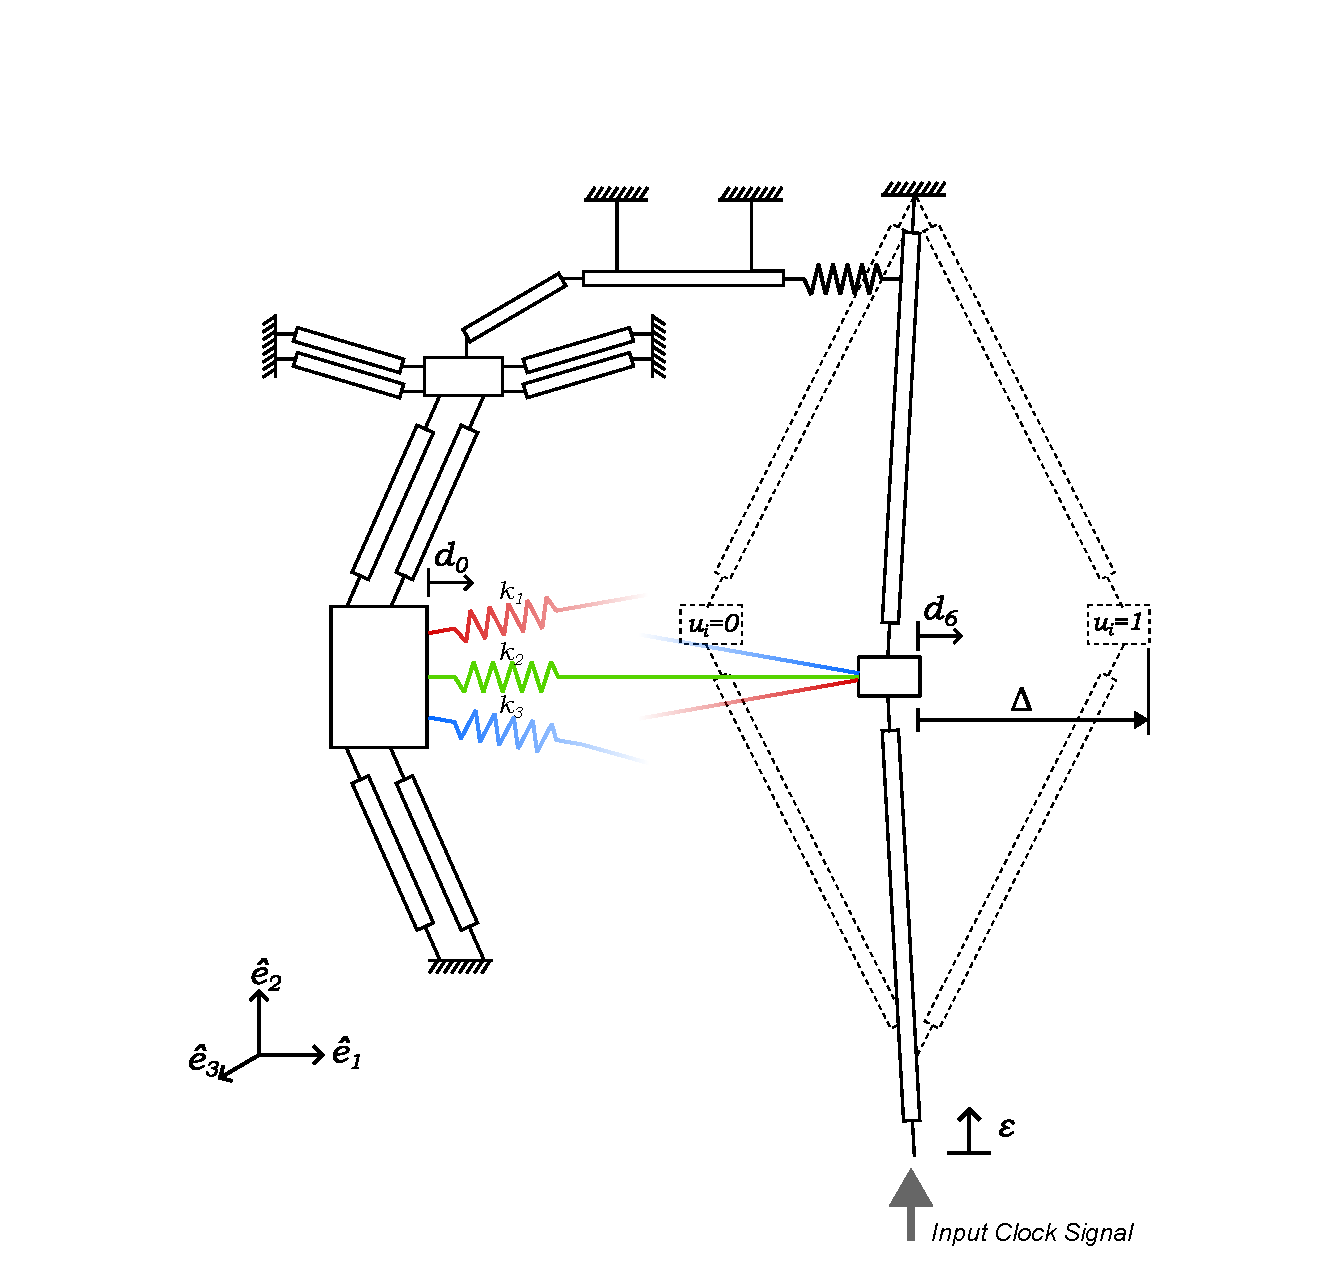
\includegraphics[width=\textwidth]{images/SVGs/PRBM.pdf}
    \caption{This is a figure.}
    \label{fig:Mechanism}
\end{figure}



\subsection*{Working Principle/Kinetics}

\autoref*{fig:Equilibria and Tension-only spring}A shows the theoretical force-displacement behaviour of the tristable element, graphing the reaction force on the tristable shuttle as a function of its horizontal displacement \(d^t\). The three stable equilibria and corresponding configuration of the mechanism are shown. 
The specific behaviour is a function of all the joint stiffnesses and the chosen geometric dimensions and proportions of the mechanism. These design parameters must be precisely calculated and calibrated to achieve the precise desired behaviour, as variation can lead to mono-stable, bi-stable, or quad-stable behaviour. The specific derivation of the force-displacement response is detailed in Appendix \ref*{sec:Compliant Mechanism Design}.

\todo{Create appendix for this derivation}

The theoretical force-displacement behavior of the coupling tension-only springs is depicted in \autoref*{fig:Equilibria and Tension-only spring}B. Specifically, the spring behaves as a linear element with stiffness \( k_i \) when its elongation is positive. For negative elongation, the spring is slack, resulting in zero force. The stiffness \( k_i \) serves as a design parameter for selecting the specific ECA rule to be implemented.

\autoref*{fig:Equilibria and Tension-only spring}C illustrates a free-body diagram detailing the forces acting upon the tristable shuttle element. Here, \( F_r \) represents the total reaction force exerted by the tristable mechanism on the shuttle, while \( F_s \) denotes the cumulative force from all non-slack coupling springs. Equilibrium is achieved when the reaction and spring forces balance: \( F_r(d^t) = F_s(d^t, d^b) \). 

\begin{figure}[h]
    \centering
    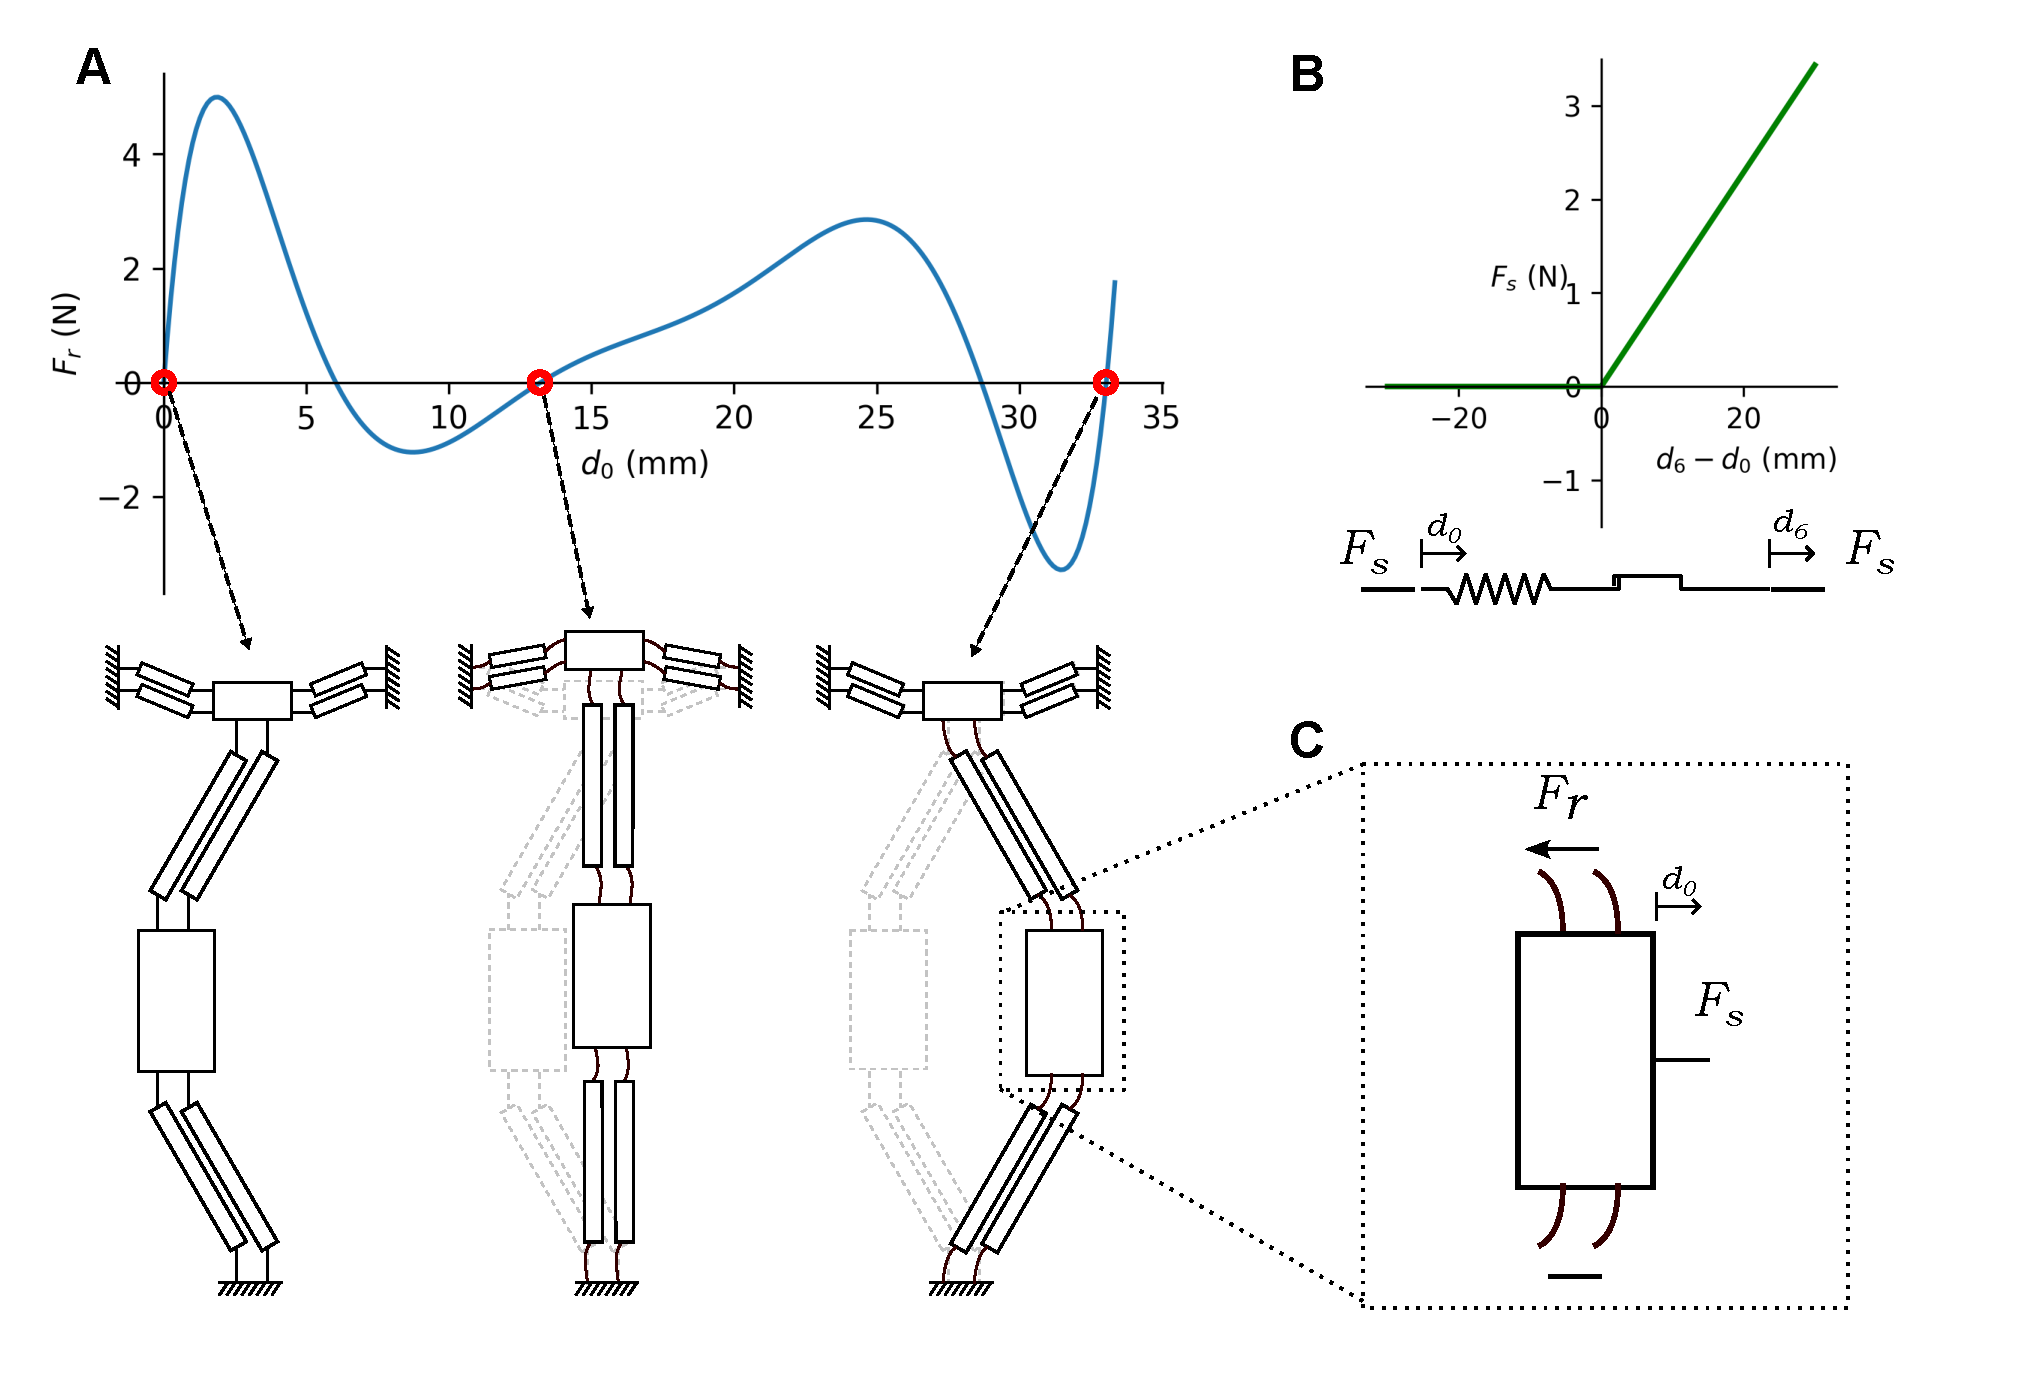
\includegraphics[width=\textwidth]{images/SVGs/Equilibria1.pdf}
    \caption{A. Force-displacement response of thethree stable equilibria and corresponding configurations of the state element. B. Force-displacement response of the tension only spring }
    \label{fig:Equilibria and Tension-only spring}

\end{figure}
    \todo{generate pdf of this figure and edit axis labels for dt etc}



In \autoref*{fig:Equilibria under actuation}, the force-displacement behavior of the unit cell is depicted under varying conditions of coupling spring activations. When the bifurcation shuttle is fixed at a displacement \( \delta \), denoted as \( d^b = \delta \), the cumulative force from the activated coupling springs is plotted alongside the force-displacement curve of the tristable element, \( F_r(d^t) \).

Equilibrium points emerge where these two force-displacement curves intersect and are represented as red dots on the difference plot. The equilibrium points correspond to the configurations where the cumulative force \( F_s \) from the coupling springs is equal to the reaction force \( F_r \) of the tristable element: \( F_r(d^t) = F_s(d^t, d^b) \).

Now, let's address the "disappearance" of the equilibrium points. An equilibrium point "disappears" when the force-displacement line of the activated coupling springs no longer intersects with specific regions of the \( F_r \) curve—specifically, the regions around its local maxima. This occurs when the slope of the force-displacement curve for the activated springs, pivoting about the point \( d^b = \delta \), not only fails to intersect but actually surpasses these local maxima regions of \( F_r(d^t) \).

In this context, snapthrough events happen as follows: the tristable element transitions from its current equilibrium state to an adjacent one depending on whether \( F_r < F_s \) or \( F_r > F_s \). This transition is triggered when the equilibrium state corresponding to the current \( F_r \) and \( F_s \) values no longer exists. This mechanical action serves as the physical embodiment of the decision boundaries in the bi-threshold perceptron.


\begin{figure}[H]
    \centering
    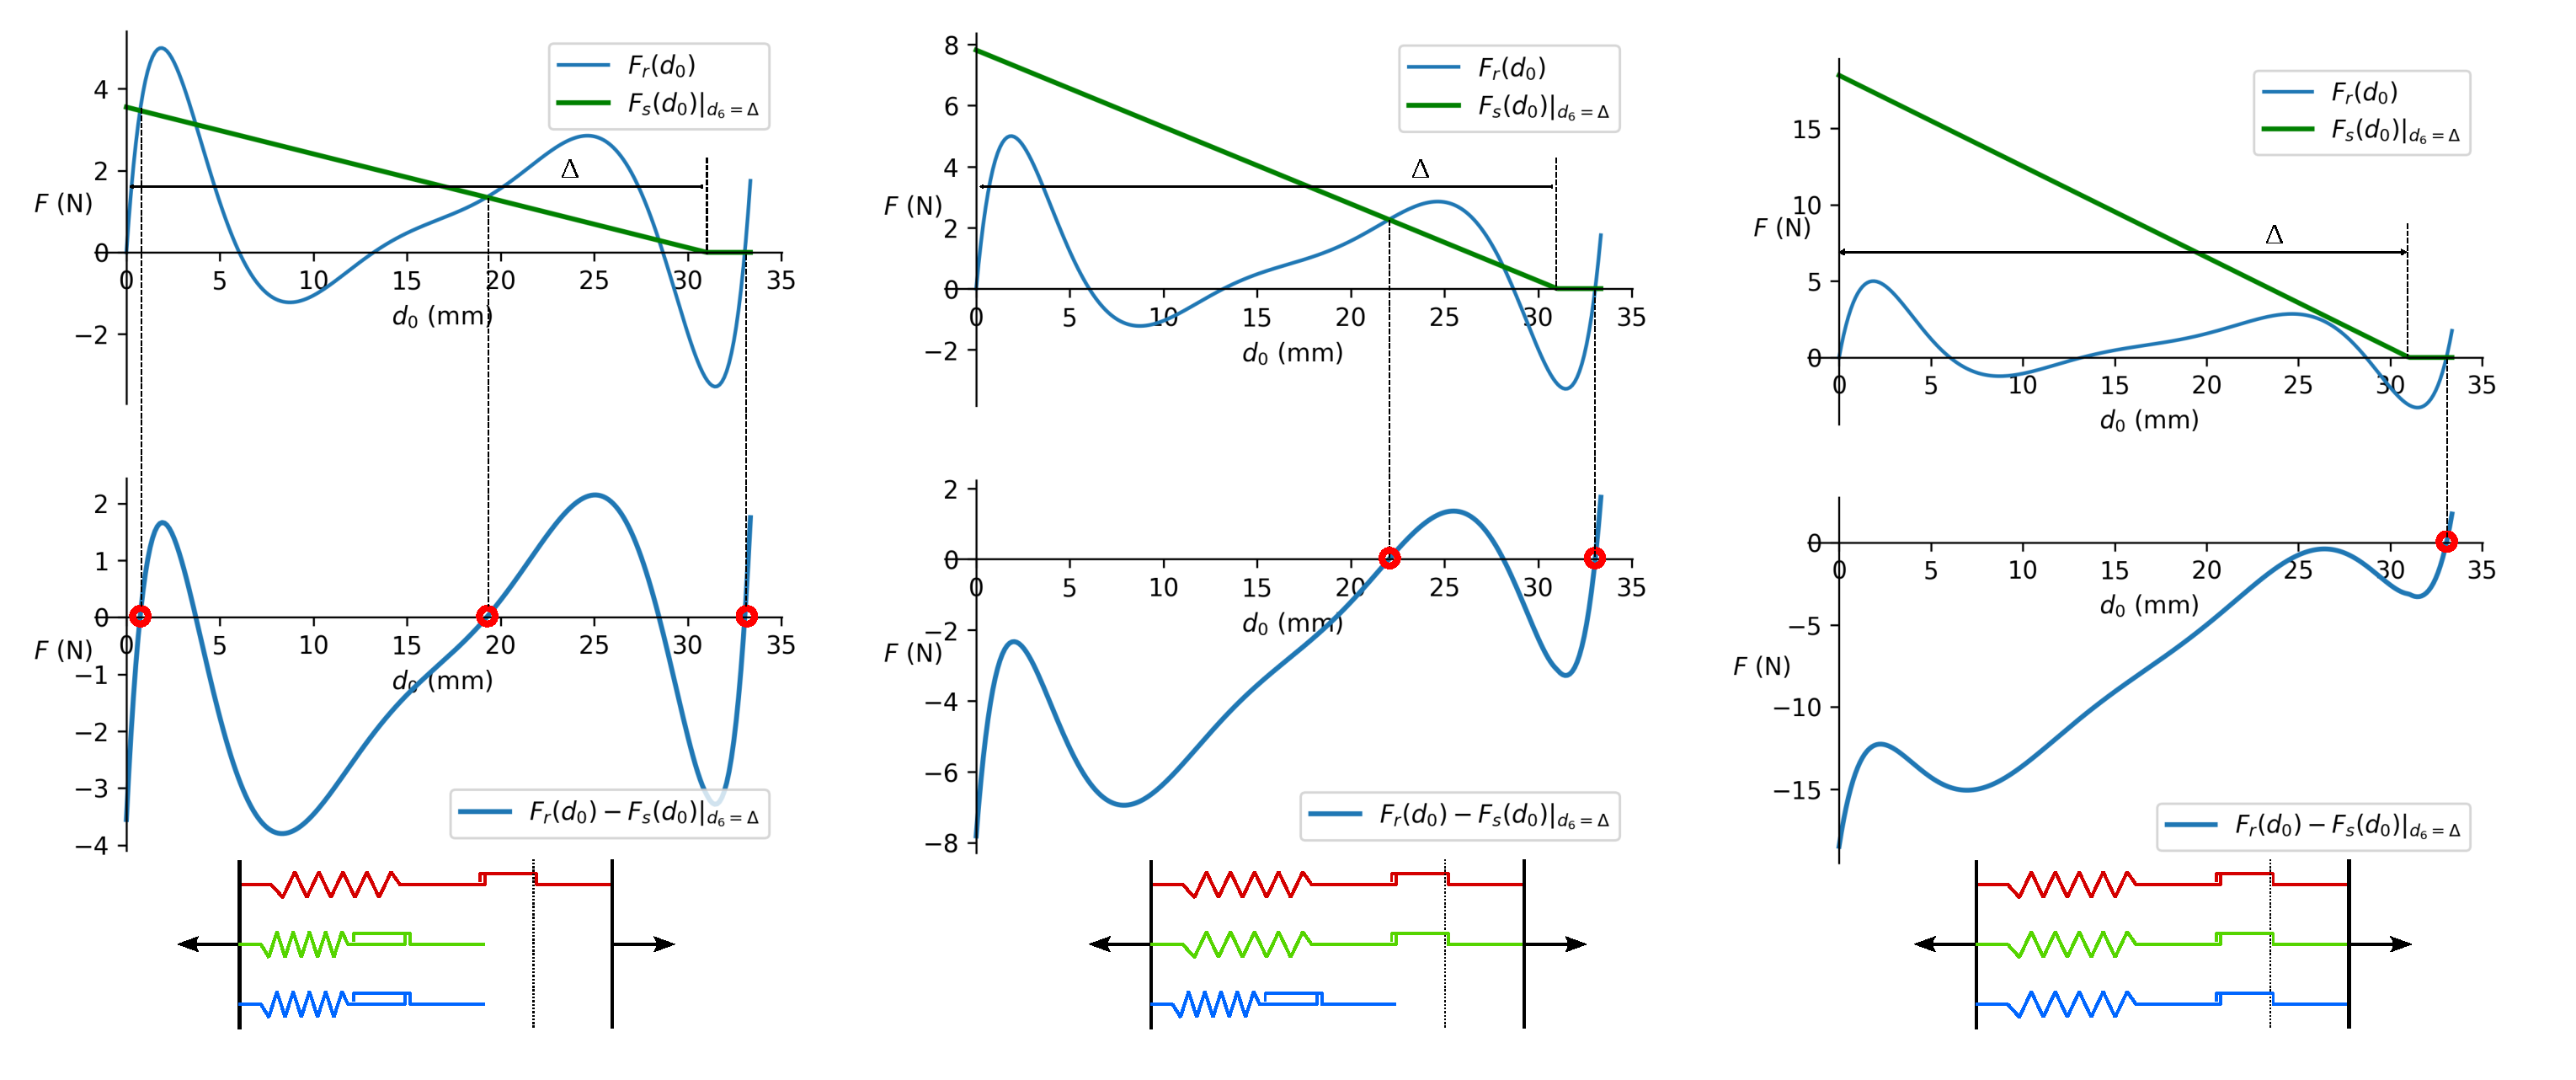
\includegraphics[width=\textwidth]{images/SVGs/Equilibria2.pdf}
    \caption{Force-displacement behavior with varying coupling spring activations. Equilibrium points, shown as red dots, emerge where the tristable element's reaction force \( F_r \) intersects with the cumulative spring force \( F_s \). Equilibria disappear when the spring force curve, anchored at \( d^b = \delta \), surpasses \( F_r \)'s local maxima, triggering a snapthrough event. This models the decision boundaries of a bi-threshold perceptron.}
    \label{fig:Equilibria under actuation}
\end{figure}

Recalling the mathematical formalism of ECA rules as bi-threshold perceptrons, we can now establish a direct correspondence between the mechanical and computational domains. In the bi-threshold perceptron model, the output state is determined by evaluating a weighted sum of inputs and comparing it against two threshold values \( T_1 \) and \( T_2 \):

\todo{add reference instead of repeating equation}

Here, \( w_i \) are the weights, and \( x_i \) are the input states from the neighborhood.

In the mechanical system, these weights \( w_i \) are analogous to the stiffness \( k_i \) of the coupling springs. The input states \( x_i \) correspond to the displacements \( d^b \) of the neighboring cells, a function of the states of their bistable elements. 
The thresholds \( T_1 \) and \( T_2 \) correspond to the critical effective stiffnesses of the cumulative active coupling springs at which the tristable element undergoes snap-through transitions. These critical effective stiffnesses are determined by the slopes of the lines that are tangent to the specific maxima regions on the \( F_r(d^t) \) force-displacement curve. These tangent lines are anchored at the point where \( d^b = \delta \) on the \( d^t \) axis.

\subsection*{Parametric determination of ECA rule}
\todo{move to methods}
Here we outline a parametric strategy for physically embodying a specific ECA rule, leveraging its geometric representation as parallel planes. The aim is to precisely calibrate the stiffness values \( k_i \) of the coupling springs and the maximum displacement \( \delta \) of the bifurcation element to manifest the desired ECA rule.

A pivotal insight is that modifying the bifurcation element's maximum displacement \( \delta \) alters the slopes of the lines tangent to the \( F_r(d^t) \) curve, as shown in \autoref*{fig:stiffness ratio}. These tangent lines are anchored at the point \( d^b = \delta \) on the \( d^t \) axis. This adjustment effectively varies the ratio between the bi-threshold perceptron's \( T_1 \) and \( T_2 \) values. Therefore, by selecting a specific \( \delta \), we can control the orientation of the separating planes, aligning them with the desired ECA rule.

Subsequently, we can determine the coupling spring stiffnesses \( k_i \) that correspond to these plane orientations, thereby completing the physical embodiment of the selected ECA rule.



\begin{figure}[H]
    \centering
    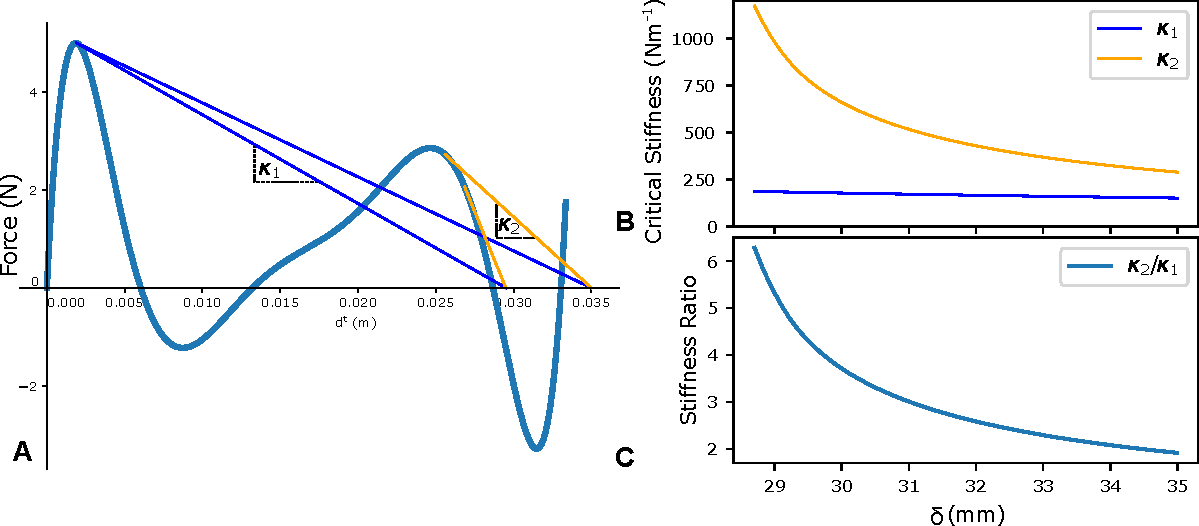
\includegraphics[width=\textwidth]{images/SVGs/stiffness_ratio.pdf}
    \caption{This is a figure.}
    \label{fig:stiffness ratio}
\end{figure}
\todo{log scale?}
\todo{show link between slopes in A and B clearer with label}

\subsection*{Implementation of Rule 110}

To demonstrate the efficacy of this parametric design strategy, we implement Rule 110 in a physical prototype. The design process is as follows:

\begin{description}
    \item[Define Rule Characteristics] Each Elementary Cellular Automata (ECA) rule can be geometrically characterized by a normal vector \( \mathbf{n} = [n_1, n_2, n_3] \) and threshold values \( T_1 \) and \( T_2 \). For example, for Rule 110, \( \mathbf{n} = [1, 2, 2] \) and \( T_1 = 1.5, T_2 = 4.5 \).
    
    \item[Compute Critical Stiffness Ratio] The ratio of the threshold values, \( \frac{T_2}{T_1} \), serves as a critical parameter in the design. For Rule 110, \( \frac{T_2}{T_1} = 3 \).
    
    \item[Determine Bifurcation Displacement] The bifurcation displacement \( \delta \) corresponding to the critical stiffness ratio is determined by consulting \autoref*{fig:stiffness ratio}C. In the case of Rule 110, \( \delta \approx 31 \, \text{mm} \).
    
    \item[Calculate Critical Stiffnesses] The critical effective stiffnesses \( \kappa_1 \) and \( \kappa_2 \) are obtained from \autoref*{fig:stiffness ratio}B, based on the selected bifurcation displacement \( \delta \).
    
    \item[Compute Coupling Spring Stiffness] The stiffness \( k_i \) of each coupling spring is then derived using:
    \[
    k_i = \frac{n_i \times \kappa_1}{T_1}
    \]
\end{description}
\todo{Explain bounds of delta}

The final mechanical parameters for a given ECA rule, such as Rule 110, are summarized in \autoref*{tab:Parametric Design Values for Rule 110}.

\begin{table}[h]
\centering
\begin{tabular}{|c|c|c|}
\hline
Parameter & Value & Units \\
\hline
\( \kappa_1 \) & 171.81 & \( \text{N/m} \) \\
\( \kappa_2 \) & 515.39 & \( \text{N/m} \) \\
\( k_1 \) & 114.54 & \( \text{N/m} \) \\
\( k_2 \) & 229.08 & \( \text{N/m} \) \\
\( k_3 \) & 229.08 & \( \text{N/m} \) \\
\( \delta \) & 31 & \( \text{mm} \) \\
\hline
\end{tabular}
\caption{Summary of Parametric Design Values for Rule 110}
\label{tab:Parametric Design Values for Rule 110}
\end{table}

\autoref*{fig:Equilibria corresponding to Rule 110} demonstrates the one-to-one correspondence between the tristable element's equilibrium configurations and the cube representation of Rule 110. Each equilibrium state is directly tied to a specific combination of activated coupling springs. The relative effective stiffness of these springs, when compared to two critical stiffness thresholds, serves as the mapping M that locates each vertex relative to the separating planes in the cube representation.
\begin{figure}[H]
    \centering
    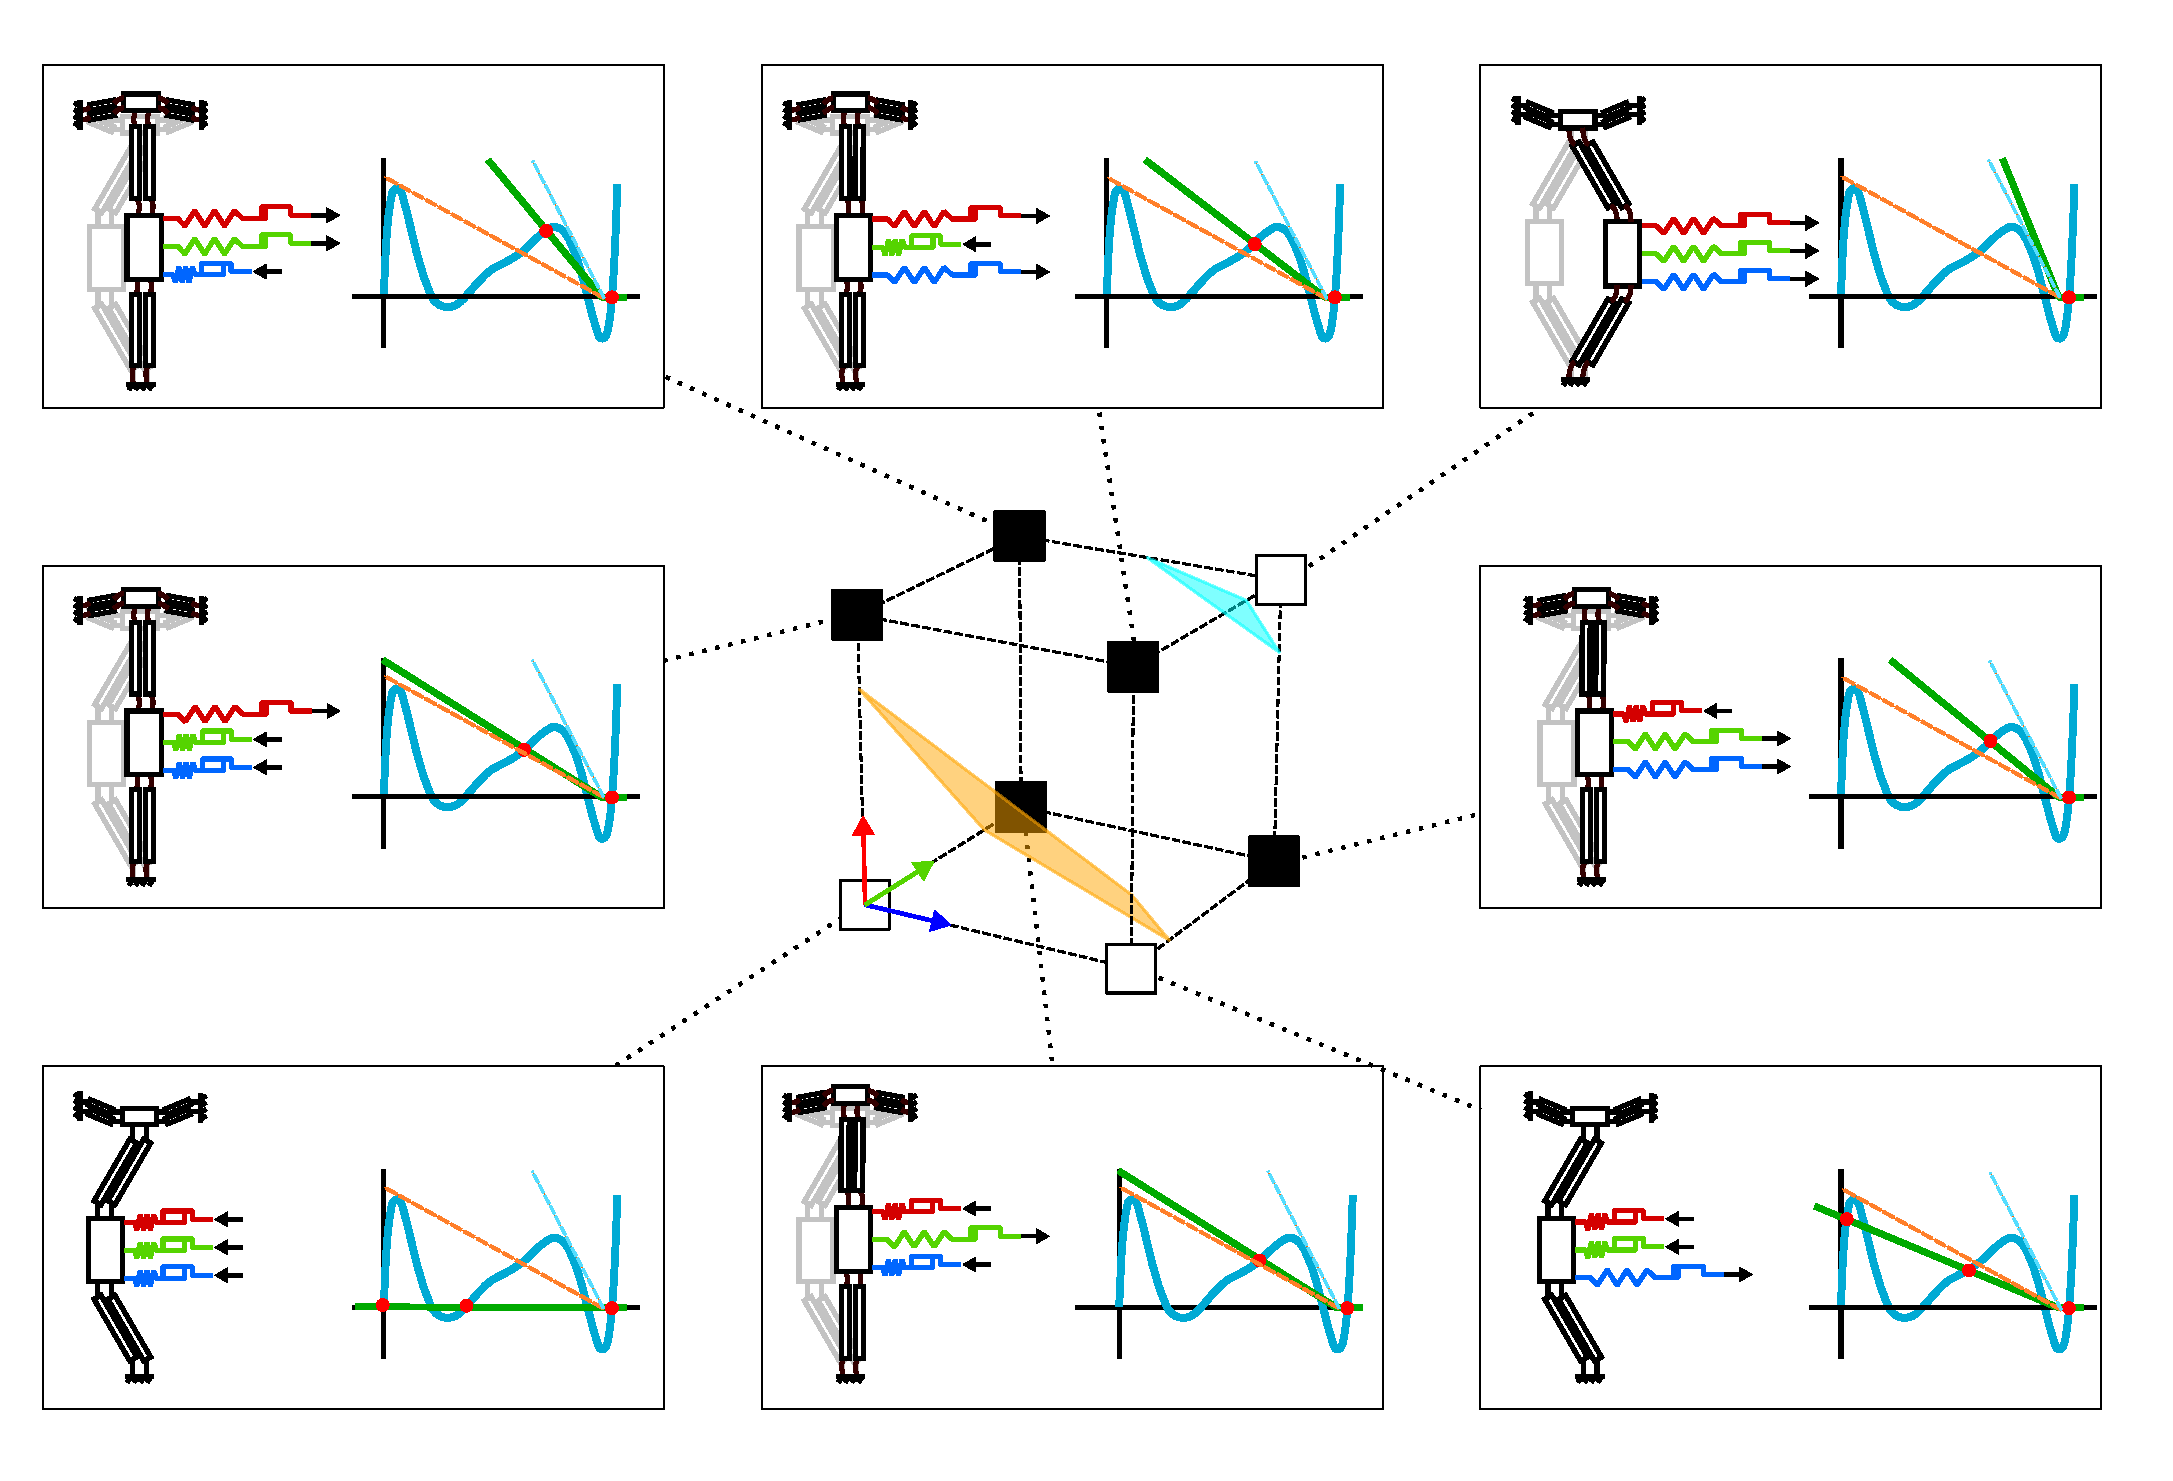
\includegraphics[width=\textwidth]{images/SVGs/Equilibria3.pdf}
    \caption{This is a figure.}
    \label{fig:Equilibria corresponding to Rule 110}
\end{figure}


\subsection*{Pseudo-Rigid Body Simulation}


The culmination and main result of the theoretical framework and concept mechanism developed thus far is a pseudo-rigid body model simulation of the unit cell and complete system, implemented in a custom Python script. The simulation implements the kinematics and kinetics of the simplified unit cell in \autoref*{fig:Mechanism}B, and models the nonlinear interaction between cells, and the simultanoeous actuation of the bifurcation mechanisms. The physical values for parameters are from \ref*{sec:Compliant Embodiment and FEA Validation}. 
\todo{explain basic procedure}
The simulation's objectives are twofold:
\begin{enumerate}
    \item To produce the force-displacement graphs that enable the parametric design strategy for implementing a specific ECA rule.
    \item To provide a computational testing ground for the system's time evolution, thereby serving as a preliminary validation of the parametric design strategy for embodying a specific ECA rule.
\end{enumerate}



The comprehensive codebase for the simulation can be found in Appendix \ref*{sec:Python Script for Pseudo-Rigid Body Simulation}.

\autoref*{fig:Simulation}A portrays a time series simulation of a 10-unit cell system. Originating from a solitary 'on' cell at the rightmost edge, the system evolves in accordance with Rule 110. The clock signal \( \epsilon \) is represented in orange. Each unit cell's bifurcation element orientation is indicative of its state—positive angle \( \theta \) equates to 'off', while negative \( \theta \) signifies 'on'. The simulation's outcomes are in harmony with theoretical projections, thereby corroborating the efficacy of the parametric design strategy, while setting the stage for further validation through FEA simulations.





\begin{figure}[H]
    \centering
    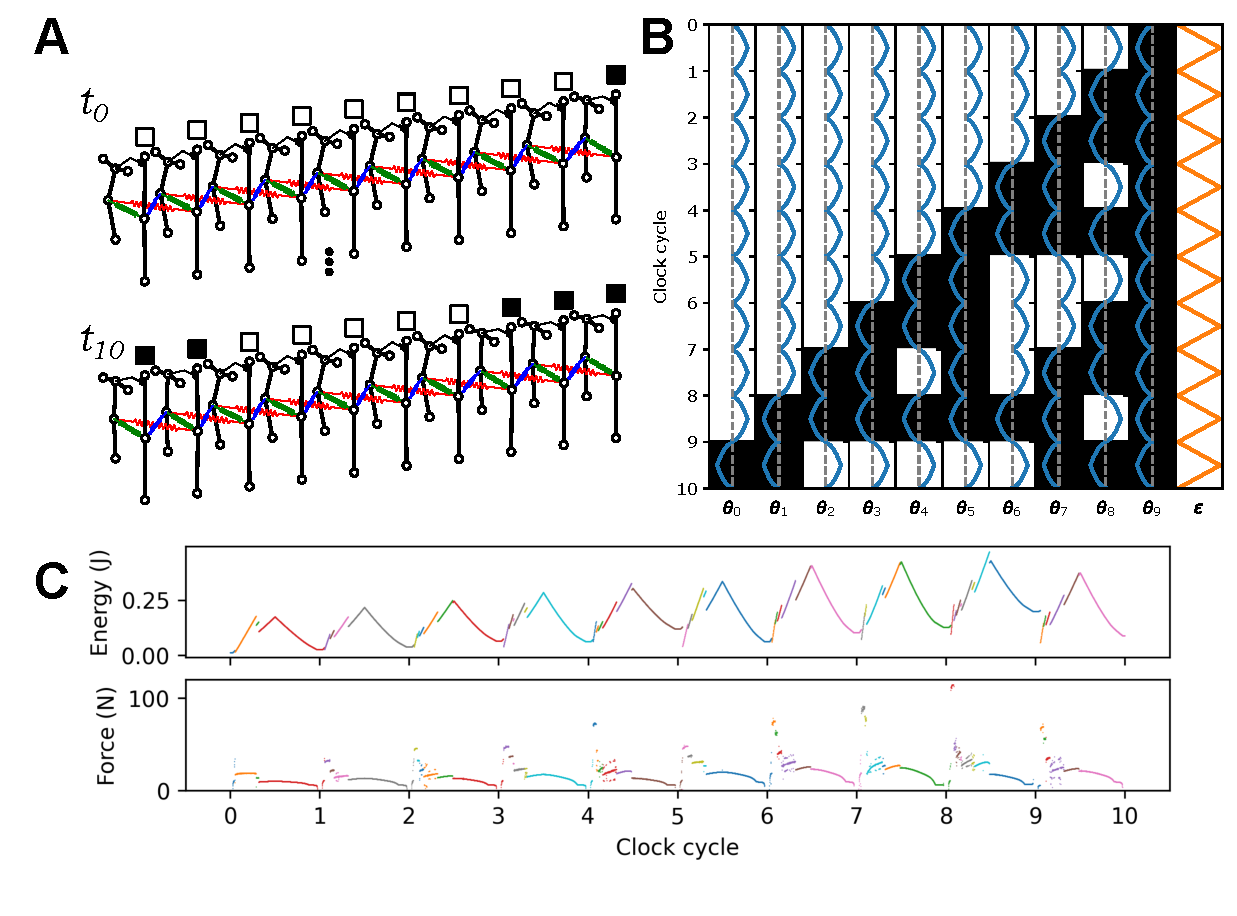
\includegraphics[width=\textwidth]{images/SVGs/Simulation.pdf}
    \caption{A. Rendering of psuedo-rigid body model at \(t_0\) and \(t_{10}\) showing arrangement of unit cells and interconnecting springs. B.Time series simulation of the system with 10 unit cells. Positive angle \(\theta\) correspons to the "off" state of the unit cell, while negative angle \(\theta\) corresponds to the "on" state. The clock signal \(\epsilon\) is shown in orange. The system evolves from a single "on" cell at the right edge of the domain according to Rule 110. C. The reaction force felt by the input displacement boundary condition \(\varepsilon\).}
    \label{fig:Simulation}
\end{figure}


\section{Discussion}

\begin{itemize}
    \item Equivalence classes of ECA rules that can be implemented
    \item Constraints of design approach
    \item Manufacturability difficulties
    \item Scalability
    \item Limitations of pseudo-rigid body model
    \item Limitations of ECAs as a computing architecture
    \item Potential applications

\end{itemize}
\section{Methods}
\subsection*{Compliant Embodiment and FEA Validation}
\label{sec:Compliant Embodiment and FEA Validation}



\subsubsection*{Parameter calculations}
Bistable element design

Tristable element design from Chen paper criteria + own criteria

Bifurcation element design

Coupling spring design

\subsubsection*{FEA Validation of Tristable Element}

Force-displacement response compared to theoretical model

Stress limits for prototype design. 

\begin{figure}
    \centering
    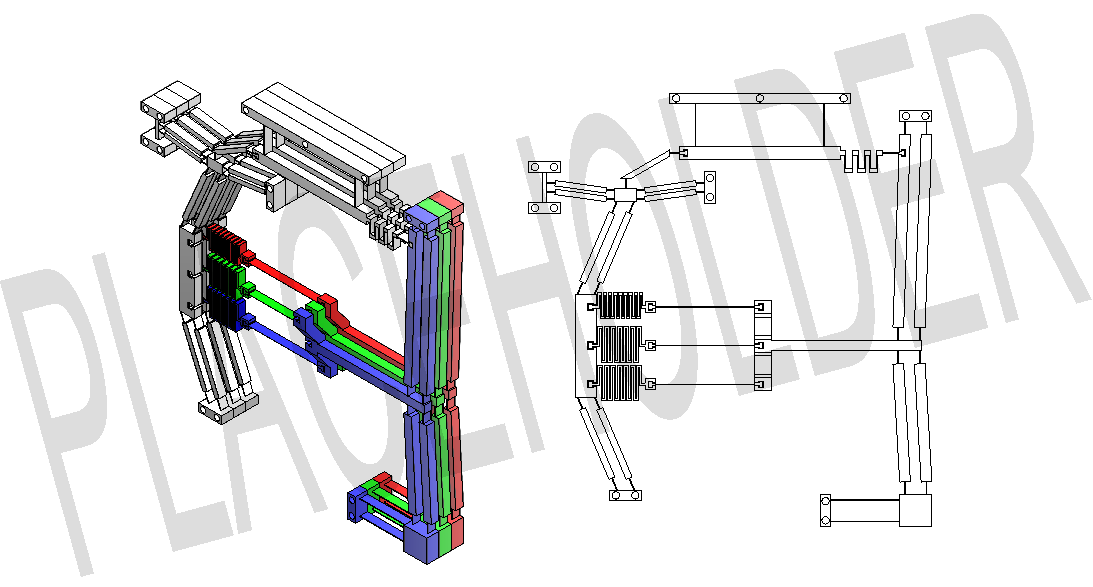
\includegraphics[width=\textwidth]{images/SVGs/v5Assembly.pdf}
    \caption{This is a figure.}
    \label{fig:Prototype}
\end{figure}
% \section{Conclusion}
% \section{References}